\documentclass{standalone}
\usepackage{tikz}
\usetikzlibrary{shapes.geometric, arrows, positioning, calc, patterns}

\begin{document}

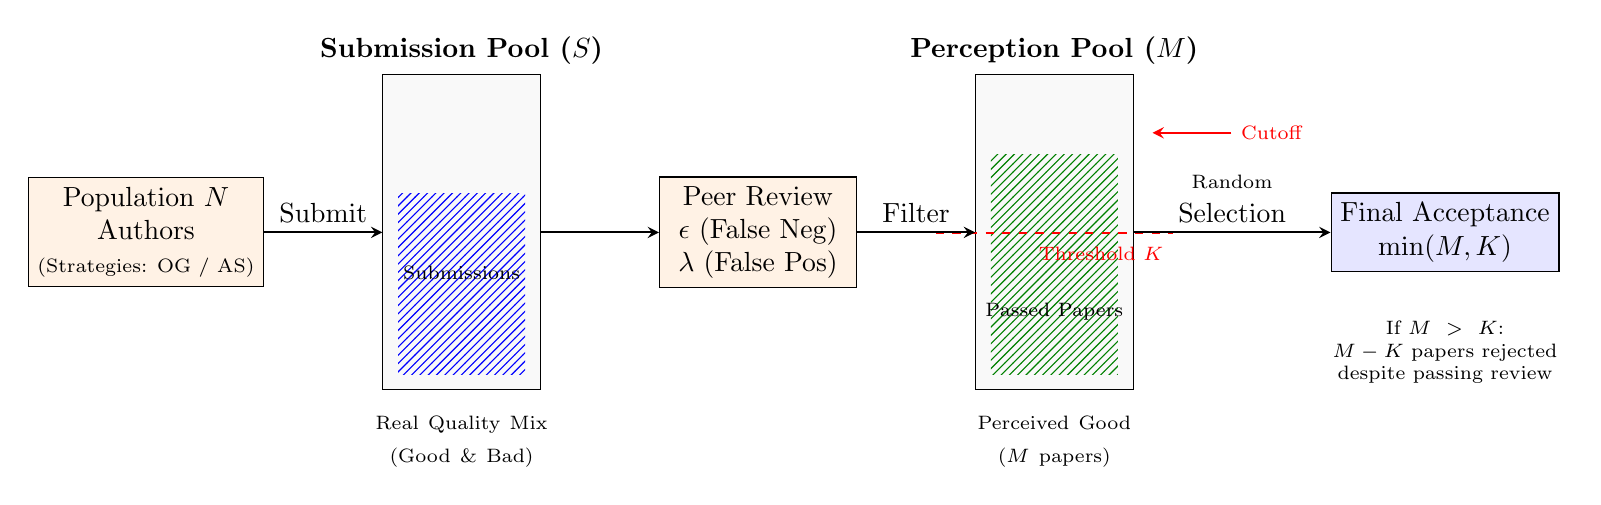
\begin{tikzpicture}[node distance=2cm, auto, >=stealth]

% Styles
\tikzstyle{process} = [rectangle, minimum width=2.5cm, minimum height=1cm, text centered, draw=black, fill=orange!10]
\tikzstyle{pool} = [rectangle, minimum width=2cm, minimum height=4cm, draw=black, fill=gray!5]
\tikzstyle{arrow} = [thick,->]
\tikzstyle{line} = [thick,-]

% --- Nodes ---

% 1. Authors & Strategy
\node (authors) [process, align=center] {Population $N$ \\ Authors \\ \scriptsize (Strategies: OG / AS)};

% 2. Submission Pool
\node (submit_pool) [pool, right=1.5cm of authors, label=above:\textbf{Submission Pool ($S$)}] {};
\fill[pattern=north east lines, pattern color=blue] ($(submit_pool.south west) + (0.2,0.2)$) rectangle ($(submit_pool.south east) + (-0.2, 2.5)$);
\node at ($(submit_pool.south) + (0, 1.5)$) {\scriptsize Submissions};

% 3. Peer Review Mechanism
\node (review) [process, right=1.5cm of submit_pool, align=center] {Peer Review \\ $\epsilon$ (False Neg) \\ $\lambda$ (False Pos)};

% 4. Perception Pool (Passed Review)
\node (percep_pool) [pool, right=1.5cm of review, label=above:\textbf{Perception Pool ($M$)}] {};
\fill[pattern=north east lines, pattern color=green!50!black] ($(percep_pool.south west) + (0.2,0.2)$) rectangle ($(percep_pool.south east) + (-0.2, 3.0)$);
\node at ($(percep_pool.south) + (0, 1.0)$) {\scriptsize Passed Papers};

% --- Threshold K (Below the line) ---
% Red Dashed Line
\draw[red, thick, dashed] ($(percep_pool.south west) + (-0.5, 2.0)$) -- ($(percep_pool.south east) + (0.5, 2.0)$);
% Text below the line
\node[text=red, anchor=north east, yshift=-0.05cm] at ($(percep_pool.south east) + (0.5, 2.0)$) {\scriptsize Threshold $K$};

% 5. Final Selection
\node (final) [process, right=2.5cm of percep_pool, align=center, fill=blue!10] {Final Acceptance \\ $\min(M, K)$};

% --- Arrows ---
\draw[arrow] (authors) -- node[above] {Submit} (submit_pool);
\draw[arrow] (submit_pool) -- (review);
\draw[arrow] (review) -- node[above] {Filter} (percep_pool);

% --- Cutoff Modification (Arrow pointing Left) ---
% Arrow from Perception Pool to Final
\draw[arrow] (percep_pool) -- node[above, align=center] (rand_sel) {\scriptsize Random\\Selection} (final);

% Cutoff Label above Random Selection, shifted slightly right
\node[above=0.2cm of rand_sel, xshift=0.5cm, text=red] (cutoff_label) {\scriptsize Cutoff};

% Arrow pointing LEFT from Cutoff label towards the Threshold line area
\draw[->, red, thick] (cutoff_label.west) -- ++(-1.0, 0);

% --- Bottom Annotations ---
\node [below=0.2cm of submit_pool, text width=2.5cm, align=center] {\scriptsize Real Quality Mix\\(Good \& Bad)};
\node [below=0.2cm of percep_pool, text width=2.5cm, align=center] {\scriptsize Perceived Good\\($M$ papers)};
\node [below=0.5cm of final, text width=3cm, align=center, font=\scriptsize] {If $M > K$: \\ $M-K$ papers rejected \\ despite passing review};

\end{tikzpicture}

\end{document}
